\documentclass[12pt]{article} 
\usepackage[francais]{babel}
\usepackage[T1]{fontenc}
\usepackage[utf8]{inputenc}
\usepackage{eurosym}
\usepackage{array}
\usepackage{graphicx}
\usepackage{fancyhdr}
\usepackage{verbatim}
\usepackage{enumerate}

\pagestyle{fancy}
\fancyhf{}
\rhead{Issidi}
\lhead{Rapport final}
\lfoot{Epita -- promotion 2020} //Insérer logo épita dans le lfoot
\rfoot{Page \thepage}


\title{Rapport final\\
		Issidi\\
		Debil.OS();}
\author{Jérémy \bsc{Beuvry}\\
		Julien \bsc{Boulicaut}\\
		Clément \bsc{Finck}\\
		Sébastien \bsc{Fleury}}

\begin{document}
\maketitle

\begin{figure}[!t]
\centering
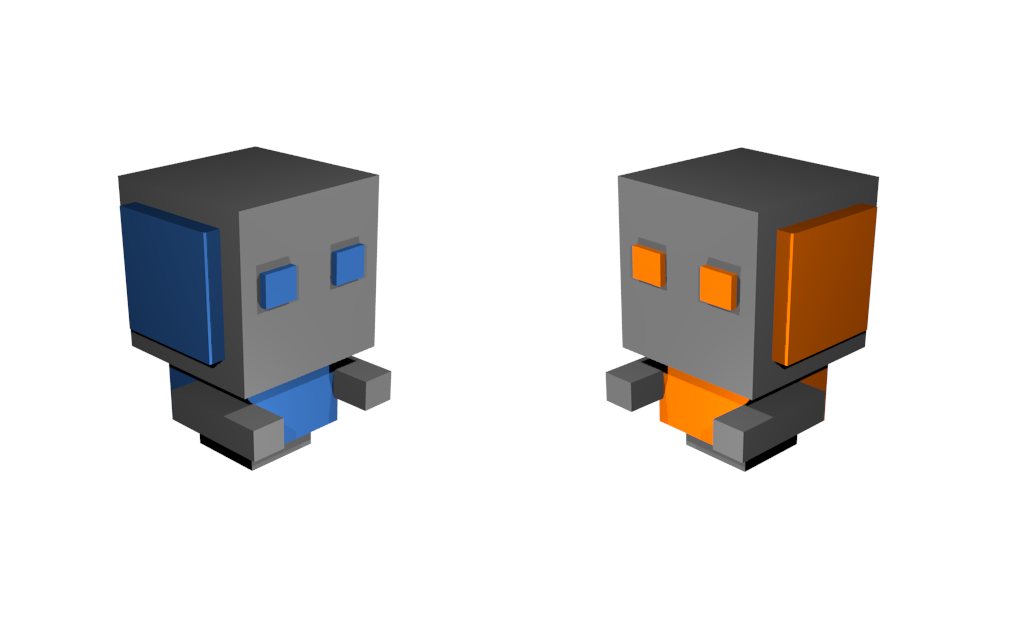
\includegraphics[scale=0.4]{front_page.png}
\caption{Des robots, personnages principaux}
\end{figure}

\newpage
\tableofcontents
\newpage
\listoffigures
\newpage

\section{Introduction}
Dans le cadre de notre première année préparatoire au sein d'Epita, 
il nous as été demandé de réaliser un projet informatique au sujet libre.

/*
**Plus de blabla sur : "comprendre la position du projet au sein 
** de notre cursus"
*/

Ainsi, notre groupe, les ''Debil.OS();'' est fier de vous présenter son 
rapport final de son magnifique, que dis-je, génialissime projet :
Issidi.

Les auteurs de ce projet sont quatre compères de première année animés
d'une motivation à toute épreuve.

Ce projet prend la forme d'un jeu de tir à la troisième personne dans
un univers post apocalyptique. Les différentes mécaniques du gameplay et
l'univers seront bien entendu détaillés dans la section adaptée.

La réalisation de ce projet Issidi nous a permit de nous confronter à
ce quii sera très probablement la réalité de notre futur métier
d'ingénieur : le travail en groupe. En effet, même si nous avons déjà eu
l'occasion de travailler en groupe au lycée ou pendant le premier semestre
, l'ampleur de ce projet nous montre l'efficacité, dans la répartition
des tâches comme dans la résolution des conflits, qui sera attendu
de nous lors de notre futur métier.

\section{Présentation}
\subsection{Présentation du projet}
\subsubsection{Introduction}

\subsubsection{Gameplay}


\subsection{Présentation des membres de l'équipe}
\subsubsection{Julien \bsc{Boulicaut}, chef de projet}
En tant que chef de projet, je tiens tout d'abord à remercier Epita qui nous
donne l'opportunité de réaliser un de nos rêves d'enfant : créer un jeu vidéo.
Passionné d'informatique depuis tout petit, j'ai commencé les tutoriels de
programmation en fin de 3ème au collège. Puis durant le lycée, je me suis contenté
de quelques programmes sur ma calculatrice ainsi que de la création de sites web.
Habitué à remplir le rôle de chef d'équipe dans la plupart des groupes auquel
j'ai participé, j'ai été choisi à l'unanimité pour assurer cette fois encore
cette fonction dans notre petite équipe. Je m'engage à maintenir la communication
entre les membres du groupe, notamment en instaurant une réunion hebdomadaire afin
d'éviter, je l'espère, d'avoir à faire des rush trop importants. Cette réunion aura
aussi pour but de faire le point au sein du groupe concernant les tâches précises 
de chacun afin d'éviter de perdre du temps en ayant des redondances dans les travaux
réalisés.

Je suis très enthousiaste concernant ce projet, et cela pour plusieurs raisons.
La première étant que j'ai la chance d'être avec trois autres personnes dont je sais
qu'elles s'investiront à 100\% dans le projet. Je suis aussi très satisfait du principe
d'Issidi que nous avons construit ensemble pendant nos pauses repas. Pour finir, je
suis très excité à la perspective d'en apprendre plus, que ce soit en C\# ou en HTML,
CSS ou encore PHP et de pouvoir enfin jouer à ce jeu auquel nous réfléchissons depuis
déjà quelques mois.

\subsubsection{Jérémy \bsc{Beuvry}}
Ayant commencé la programmation depuis déjà 4 ans, je mettrai à profit les compétences
apprises lors de projets personnels, nombreux mais pas finis. En effet, ce projet issu
d'une longue réflexion au sein de notre groupe et avec un grand potentiel me permettra
dans ce projet de grande envergure d'utiliser intelligemment ce que j'ai appris précédemment,
dans un groupe avec une excellente entente en son sein. De plus, ce projet m'apprendra
le travail en équipe, qui est une compétence fondamentale dans le monde d'aujourd'hui,
ainsi que l'apprentissage d'un nouveau langage qu'est le C #, qui m'était totalement
inconnu avant mon entrée à Epita. Ainsi, c'est avec un énorme sourire aux lèvres que
je m'apprête à commencer ce projet. 

\subsubsection{Clément \bsc{Finck}}
J'ai très peu codé dans ma vie mais j'ai toujours eu envie de participer à ce genre de
projet et Epita me donne l'opportunité de pouvoir participer enfin à ceci. Créer un jeu
vidéo a toujours fait partie de mes rêves même si je n'ai jamais réussi à passer le cap
tout seul. Je saisis cette occasion pour pouvoir montrer ce que je peux faire en me
donnant à 200%. De plus je suis très confiant par rapport à mon groupe car je sais
que tous autant qu'ils sont, ils seront se donner à fond afin que celui-ci soit le
meilleur possible. J'ai très envie de pouvoir aider mon équipe autant que possible et
je pense vraiment que ce projet sera une réussite. Je suis très content de l'idée
centrale de notre projet car je la trouve très originale et efficace car je ne connais
aucun jeu basé sur un tel gameplay. De plus, je pense que notre équipe sera un très 
bon moyen pour moi d'améliorer mes connaissances en codage et cela me ravit. 

\subsubsection{Sébastien \bsc{Fleury}}
Pendant longtemps j'ai voulu automatiser plusieurs tâches sur mon ordinateur, ce qui
m'amena à apprendre en 3\ieme la programmation. C'est donc depuis 4 ans que je travaille
régulièrement sur le framework .NET et plus récemment Java. J'ai eu la chance aussi de
pouvoir travailler sur d'autres types de compilateur avec une API bien moins complète
et intuitive. Ce projet m'enseignera une meilleure pratique du travail d'équipe, plus
importante que celle que j'ai actuellement et l'utilisation d'un autre moteur graphique,
ayant utilisé XNA, nativement celui du .NET. J'ai donc comme tout notre groupe beaucoup
à apprendre en travaillant sur ce projet. J'ai de plus la chance de travailler avec des
camarades non seulement très impliqués dans le projet, mais aussi et surtout très sympathiques,
ouverts aux suggestions et capables de trouver des solutions aux problèmes.



\section{Bilan du projet}
Bilan sur nous et notre groupe.
Pas le même bilan au sein du groupe.
On ne s'agresse pas (dommage...)

\section{Conclusion}

\section{Bibliographie}
LOL... (en plus faut la commenté)

- docs.unity.com
- stackoverflow.com